\section{Line Detection}
\label{sec:lineDetection}

Many line detection algorithms stem from the road domain, to detect lanes.
This is done for autonomous or safety systems for cars.
Most algorithms are trained on datasets like TuSimple \cite{tuSimpleDataset} or CULane \cite{cuLaneDataset}, which include images taken in the front view of cars.
While TuSimple is captured on US highways CULane's images are from Beijing.
\autoref{fig:tusimpleExample} shows examples of TuSimple.

\vspace{1cm}

\begin{figure}[H]
    \centering
    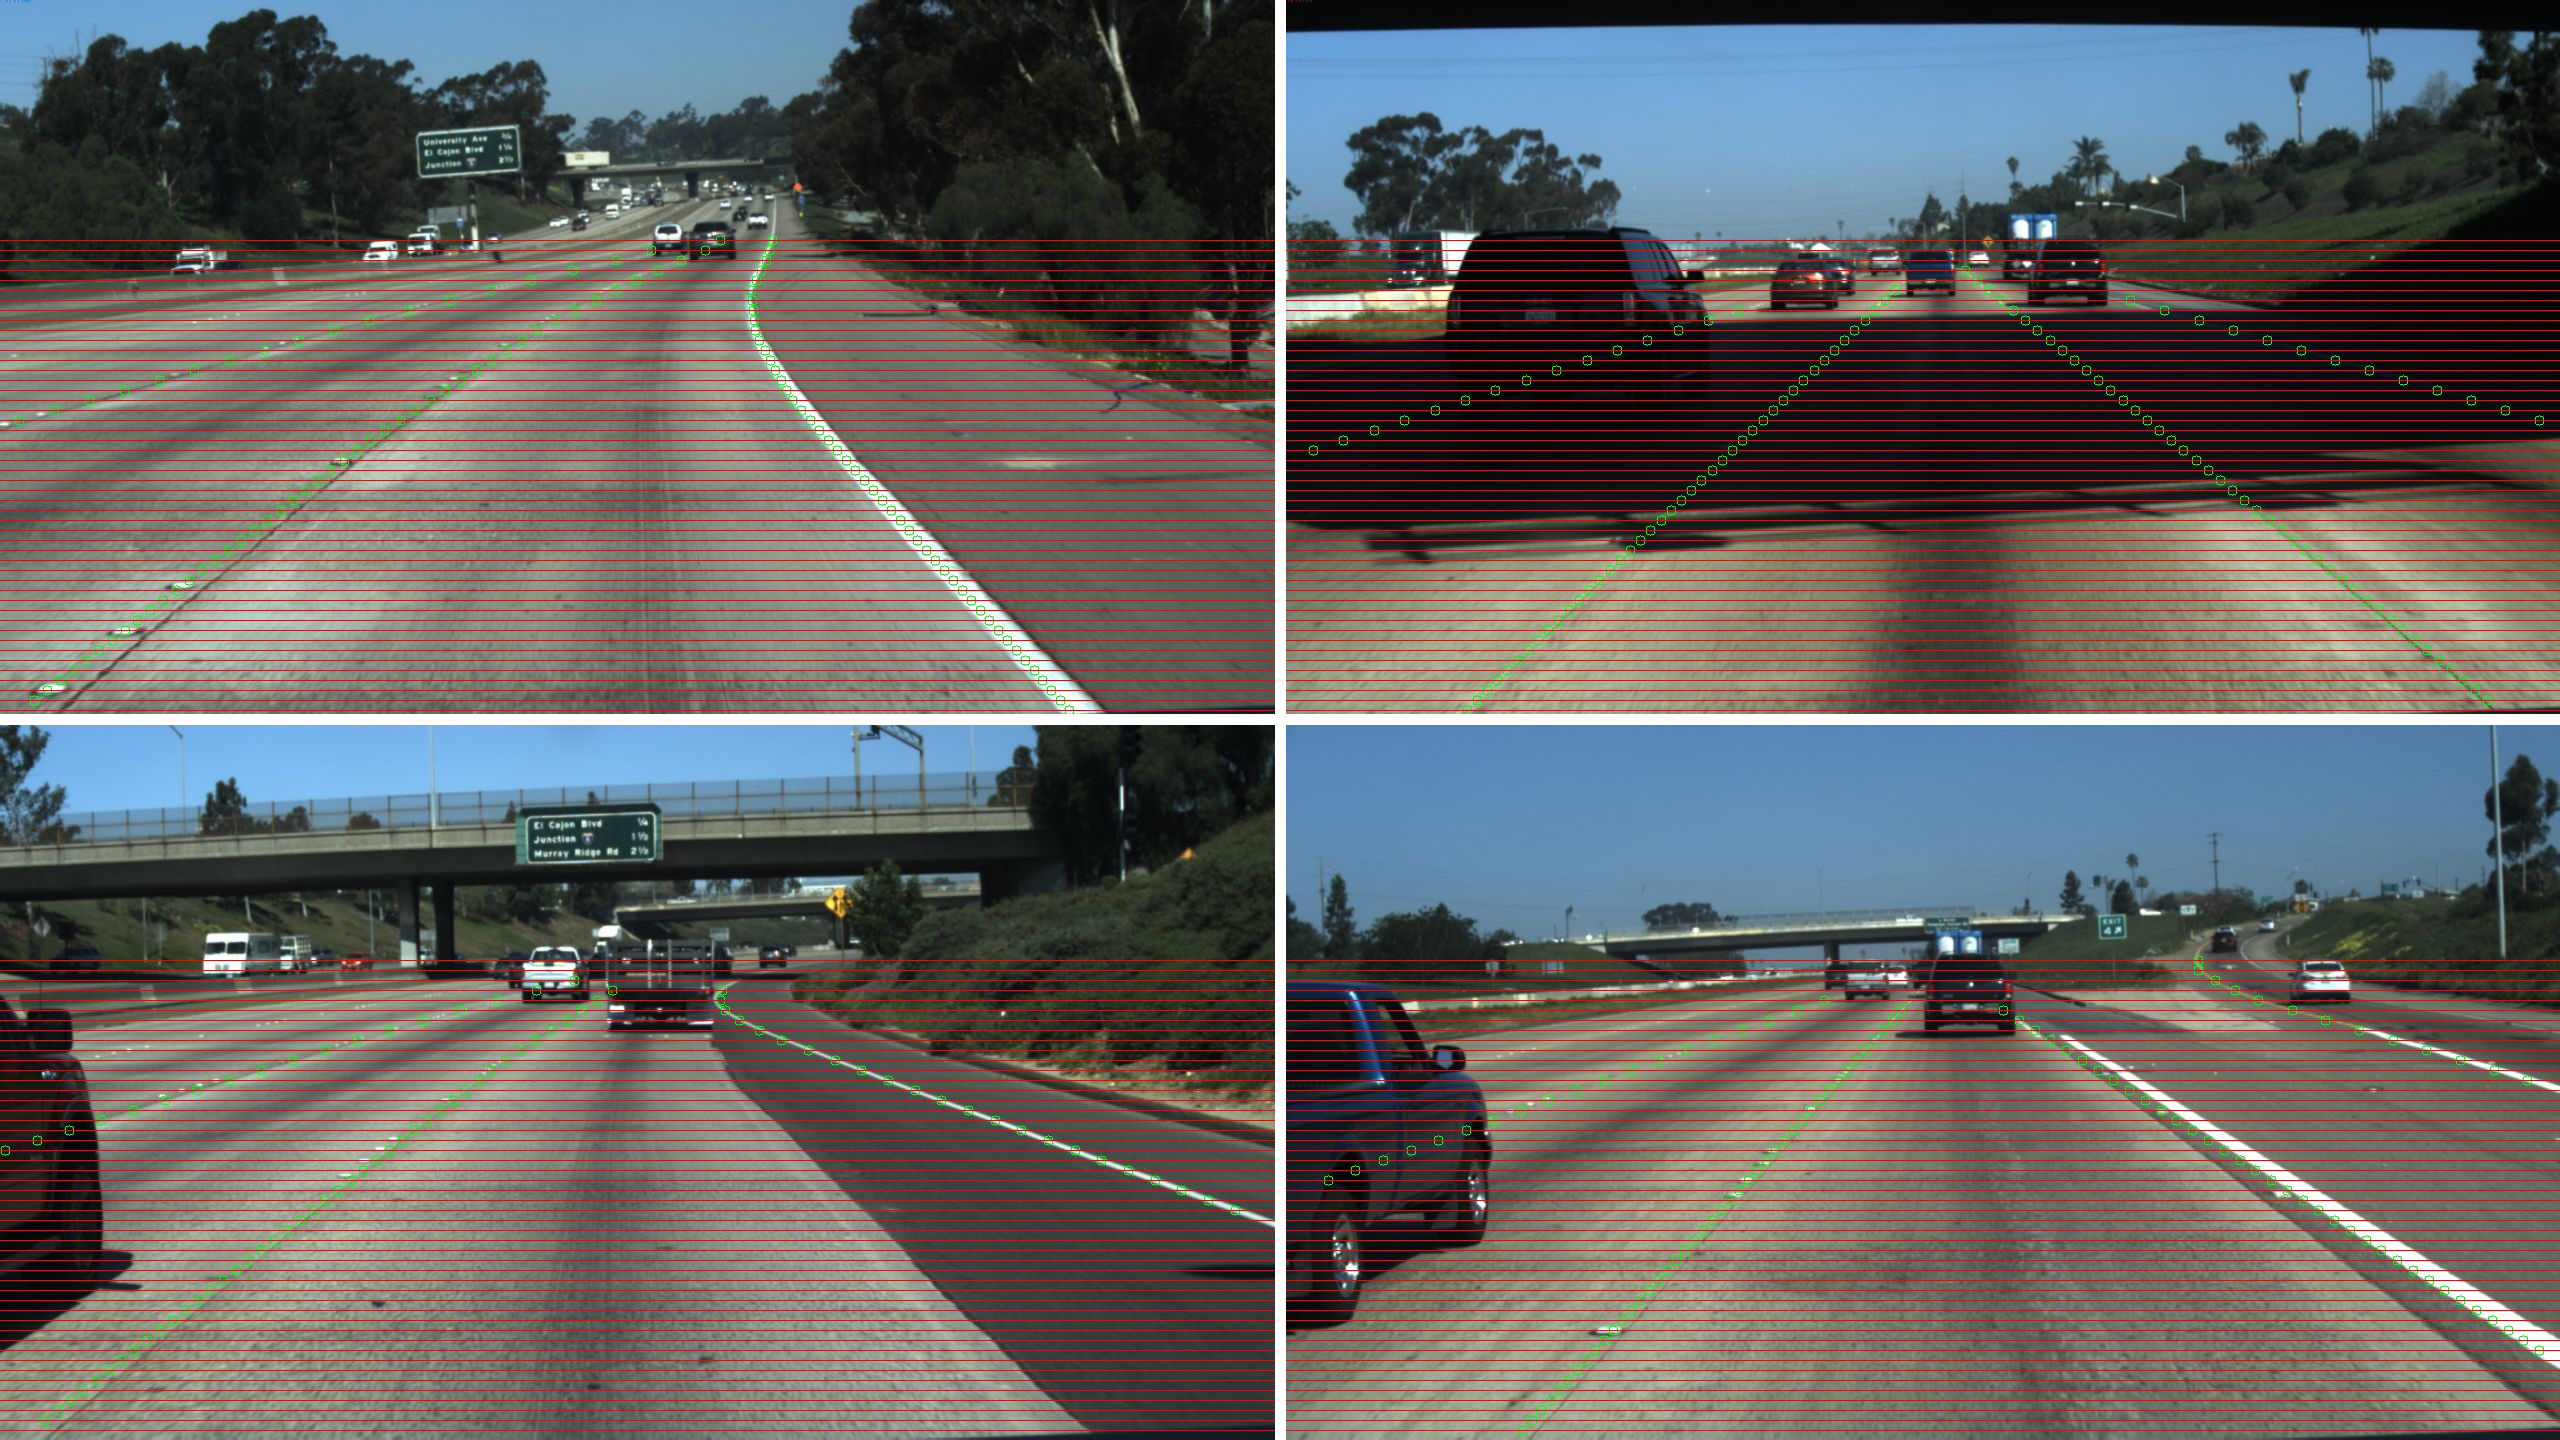
\includegraphics[width=\linewidth]{PICs/lineDetection/tusimple_example.jpg}
    \caption{Example Images of TuSimple with annotations \cite{tuSimpleDatasetExampleImage}. Red lines are horizontal anchor lines. Green circles mark image coordinates, where road lanes and anchor lines intersect.}
    \label{fig:tusimpleExample}
\end{figure}

\vspace{1cm}

\cite{LaneDetectionCascadedCNNs2019} proposed one of the first lane detection approaches on TuSimple.
The proposed method detects lanes and classifies the kind of lane.
Two cascaded CNNs are utilized, the first one is an encoder-decoder network for instance segmentation and the second one is a classification network.

However encoder-decoder structures are very similar to the techniques used for semantic segmentation.
Other structures for lane detection include key point extraction, grid systems, or polyline regression.

\textbf{Keypoint detection on the road}

\cite{LineCNN2020} proposed Line-CNN, which includes a ResNet backbone and an introduced Line Proposal Unit.
The model suggests a series of lines to locate road lanes.
After the proposal, the line with the highest confidence score is fitted with horizontal offsets to match the actual lane.

\cite{CurveLaneNAS2020} proposed a network, that predicts road lanes with the horizontal offsets from a pre-defined vertical anchor.
Additionally, \cite{CurveLaneNAS2020} utilized a \ac{NAS} to find the optimal architecture for this task.

Similar to Line-CNN, the method proposed in \cite{KeepEyesOnLane2021} also proposes lines with confidence scores and fits the resulting output with horizontal offsets.
The novelty of this approach is in an introduced attention mechanism based on anchors.
This added module results in higher accuracy and a much faster model with speeds up to 250 \ac{FPS}.

Another approach that uses key points is introduced in \cite{GANet2022}.
This architecture utilizes a Lane-aware Feature Aggregation module to strengthen the connection between neighboring key points and archives state-of-the-art performance.

\textbf{Grid system}

An approach that uses grid systems is proposed by \cite{laneDetectionGrid2020}.
Here a row-wise classification is done for a predefined number of grids.
The number of grids is equivalent to the number of lanes that can be detected.

\textbf{polyline regression}

A regression approach is proposed in \cite{PolyLaneNetRoad2021}, that predicts the polynomials of lanes.
ResNet and EfficientNet backbones are used to extract features, that are then used to forecast lines.
Each line includes the coefficients of a polynomial, a starting parameter, and a confidence score.
Additionally, a shared horizon line is predicted, where all polylines end.
Compared to other state-of-the-art approaches, \cite{PolyLaneNetRoad2021} proposes a computationally efficient method with speeds up to 115 \ac{FPS}.
While accuracy is lower than with other methods, it still is comparable.

\cite{DetectingLanesWithBezierCurves2023} proposed an approach that predicts the parameters of a cubic Bezier curve.
This curve is fitted in the area defined by four control points.
A typical backbone like ResNet with additional feature flip fusion modules is utilized.
After a pooling and two convolutional layers, the model outputs the prediction.
Compared to polynomial fitting the approach proposed in \cite{DetectingLanesWithBezierCurves2023} is superior.

\textbf{rail domain}

Even though much has been done in the road domain, and the rail domain is usually not considered, some research has still been conducted to adapt lane detection algorithms for trains.


Some of the mentioned research approaches utilize key point extraction to detect lanes.
\cite{topologyGuidedRailDetection2022} adapts this concept with semantic segmentation as pre-processing for detecting rails.
The technique can be divided into four steps.
Firstly, there is image preprocessing, in which a semantic segmentation network filters out the rails in an image.
Additionally, an inverse perspective transformation is utilized to bring the binary mask into a bird-eye view for easier image handling in further steps.
Secondly, rail-track discretization, in which a key point extraction, a connectivity judgment, and a breakpoint connection are used to divide the cluster of one-class pixels from the binary segmentation mask into different rails.
Thirdly, the rail lane reconstruction where the data from the second step is combined with the bird-eye view from the first to connect the extracted key points to obtain a complete rail lane instead of discrete points.
In the final step, rails are matched in pairs, to receive the final output.
However, no distinction is made between the train's rail and other rails.
Two additional issues lay in the complex data processing of this approach.
On the one hand, it is stated that the algorithm's accuracy relies too much on the semantic segmentation used at the start.
On the other hand, no records of speed are available.
\cite{topologyGuidedRailDetection2022} proposes an intricate approach with complex cascaded algorithms that easily could exceed real-time requirements.


Another state-of-the-art approach to filtering out rails is to divide the output into grids \cite{li2022rail}.
This technique is also adapted from the road domain from \cite{laneDetectionGrid2020}.
Each rail is predicted in a separate grid and the number of rails is predefined with the hyperparameter $C$, as shown in \autoref{fig:gridLineDetection}.
In each grid, a row-wise classification problem is solved, where the target class corresponds to the cell that encompasses the target rail.
After that, the grid system with the predicted cells is translated into image coordinates to calculate the final output.
The architecture is shown in \autoref{fig:gridLineDetection}, which also shows the focus on detecting all rails in an image.
This approach relies only on the feature extractor and therefore does not need a decoder.
In 2024 this approach is also used by TEP-Net \cite{tepNet2024} with just the train's own two rails for state-of-the-art comparison.

\begin{figure}[H]
    \centering
    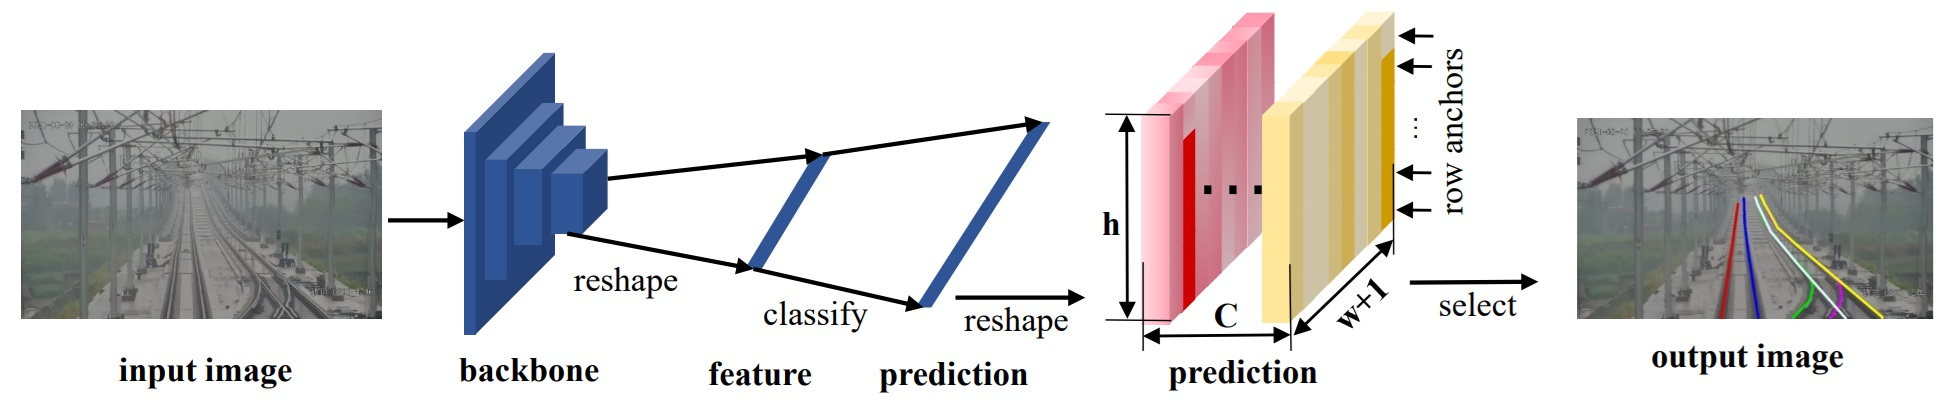
\includegraphics[width=\linewidth]{PICs/lineDetection/gridDetection.jpg}
    \caption{Rail detection with Gridsystem \cite{li2022rail}. Hyperparameters: $C$ is the number of rails (number of grids). $h$ is the number of cells vertically. $w+1$ is the number of cells horizontally with an additional column for a background class, when no rail is detected in a row.}
    \label{fig:gridLineDetection}
\end{figure}

